% Présentation de TeX et LaTeX
\small

\section{A \TeX\ and \LaTeX\ Presentation}

\subsection{What is \TeX\ and \LaTeX?}

% Qu'est-ce que TeX?
\begin{frame}{What is \TeX?}
	\begin{columns}
		\begin{HEClegende}{Donald Knuth}
			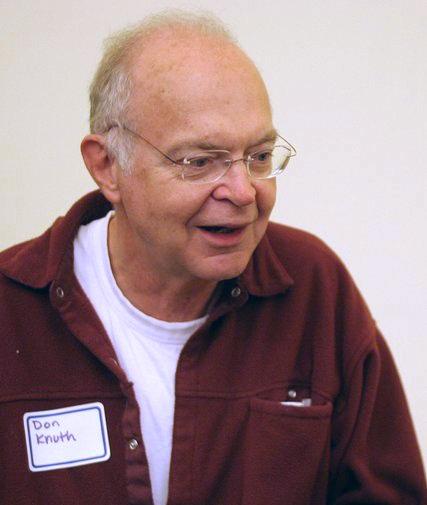
\includegraphics[width=.9\textwidth,keepaspectratio=true]{KnuthAtOpenContentAlliance.jpg}
			
			{\tiny\faCreativeCommons\ Jacob Appelbaum, 2005}
		\end{HEClegende}
		\begin{HECcontenuLegende}
			\begin{itemize}
				\item A typesetting system created by Donald Knuth.
				\item ``The most powerful formatting program for producing book-quality text of scientific and technical works.''\footnote{Kopka \& Daly, p. 6}
				\item A mature, stable, complete, bug-free system.
				\item A set of primitive commands perfect for typographic and programmatic functions.
				\item ``\emph{typesetter-level program}''
			\end{itemize}
		\end{HECcontenuLegende}
	\end{columns}
\end{frame}

% Qu'est-ce que LaTeX?
\begin{frame}{What is \LaTeX?}
	\begin{columns}
		\begin{HEClegende}{Leslie Lamport}
			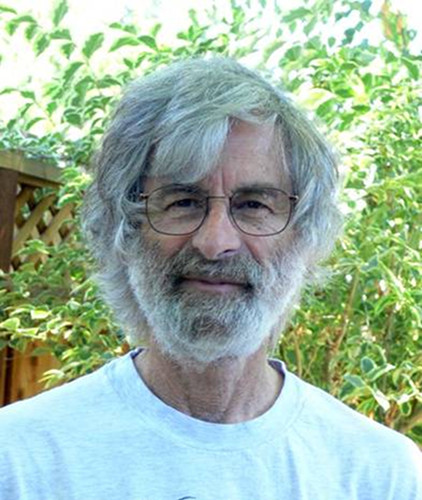
\includegraphics[width=.9\textwidth,keepaspectratio=true]{Leslie_Lamport.jpg}
		\end{HEClegende}
		\begin{HECcontenuLegende}
			\begin{itemize}
				\item A set of markup commands created by Leslie Lamport to facilitate \TeX's use.
				\item Doesn't require any knowledge of typography in general and \TeX\ particularly.
				\item Typographic and logical markup language used to set the text layout (like HTML).
				\item Cross-platform language, identical from one operating system to the other and extensible with packages.
				\item ``\emph{author-level program}''
			\end{itemize}
		\end{HECcontenuLegende}
	\end{columns}
\end{frame}

\subsection{\LaTeX\ Document Creation Process}

% Rédiger avec une nouvelle perspective
\begin{frame}[c]{Writing with a new perspective}
	
	\begin{itemize}
		\item You write your document in plain text and you use commands to describe 
			\textbf{what the text is} and \textbf{not what it should look like}.
		\item You focus on your \textbf{content}.
		\item You let \LaTeX\ do its work, that is taking care of the \textbf{container}.
	\end{itemize}
	
\end{frame}

% Processus de création d'un document LaTeX
\begin{frame}[c]{\LaTeX\ Document Creation Process}
	\Huge
	\begin{minipage}[t]{0.25\linewidth}
		\centering
		\faFileTextO
	\end{minipage}
	\hfill\faArrowRight\hfill
	\begin{minipage}[t]{0.25\linewidth}
		\centering
		\faCogs
	\end{minipage}
	\hfill\faArrowRight\hfill
	\begin{minipage}[t]{0.25\linewidth}
		\centering
		\faFilePdfO
	\end{minipage}

	\begin{picture}(0,0)
		\footnotesize\thicklines\color{bleuFonceSecondaire}
		\onslide<2>\put(0,-10){\dashbox{1}(35,40)[b]{\parbox{.2\textwidth}{\centering\textbf{writing and markup with a text editor\smallskip}}}}
		\onslide<3>\put(54,-10){\dashbox{1}(35,40)[b]{\parbox{.2\textwidth}{\centering\textbf{compilation with a \TeX\ compiler from the command line\smallskip}}}}
		\onslide<4>\put(108,-10){\dashbox{1}(35,40)[b]{\parbox{.2\textwidth}{\centering\textbf{visualization with an external reader\smallskip}}}}
	\end{picture}
\end{frame}

% Quelques choses simple à réaliser avec LaTeX
\begin{frame}{Some Things Done Simply with \LaTeX\ldots}
	\framesubtitle{\ldots\ and not necessarily with a word processor}
	
	\begin{itemize}
		\item Title page
		\item Table of contents
		\item Page numbering
		\item Figures and tables: display on a page, numbering, reference
		\item Equations: display, numbering and reference
		\item Citations and bibliographies
		\item Hyphenation
		\item Two-sided documents
	\end{itemize}
\end{frame}

% Les outils dont vous aurez besoin
\begin{frame}[c]{Tools you'll need}
	
	\begin{itemize}
		\item A \TeX\ distribution
			\begin{itemize}
				\item \href{https://www.tug.org/texlive/}{\TeX\ Live} (Windows and Unix/Linux)
				\item \href{https://www.tug.org/mactex/}{Mac\TeX}, derived from \TeX\ Live (Mac OS)
				\item \href{https://miktex.org/}{MiK\TeX} (Windows, Mac OS and Unix/Linux)
			\end{itemize}
		\item An integrated writing environment
			\begin{itemize}
				\item \href{https://en.wikipedia.org/wiki/Comparison_of_TeX_editors}{Too many} to list them all\ldots
				\item The library uses and recommends \href{https://www.texstudio.org/}{%
					\TeX Studio}
			\end{itemize}
		\item A command line terminal
	\end{itemize}
\end{frame}